\chapter{Introduction to Messaging} 

Before we can understand what Apache Kafka is, we first need to
know how messaging basically works and what a message broker is. Also there are other
important terms related to messaging we want do declare. 

\begin{figure}[H]
    \centering
    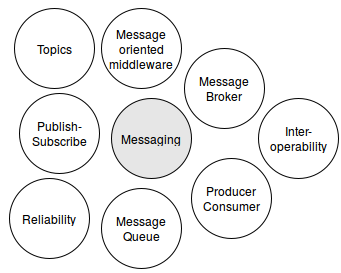
\includegraphics[width=0.35\textwidth]{images/messaging-intro.png}
    \caption{Messaging terms}
    \label{fig:MBig:the-log}
\end{figure}

In advance, we start with the definition of the term distributed systems. A distributed system
consists of a collection of multiple autonomous components, connected through
network, which enables to coordinate  (e.g. computers) their activities and to
share resources. To a user, these systems are perceived as a single, integrated
computing facility. Other than centralised systems, distributed systems has it's
advantages in economics, performance and scalability and reliability. In fact,
this approach allows us to build reliable applications, scaled using low cost
computers and thus can serve massive performance needs whether on demand or
continuously.\cite{POSA1}\cite{TAN06}
\todo{gls?
}
\section{Message Oriented Middleware}
\label{intro-messaging-mom}
Introducing an intermediate component between distributed
clients, messaging reduces the close coupling of other communication styles just
based on \gls{Socket}s or RMI. This additional component can be named as
Message-Oriented Middleware (MOM) and is all about passing \gls{Msg}s in any
format from one application to another whereas the parties do not need to know
each other directly. Thereby the main characteristic of a MOM is that its
supports a storage capacity which leads to a persistent way of communication where it is
not required that the collaborating endpoints are active during the entire
transmission of a message. This loose coupling in time is achieved by
working with queues as data structure (first-in-first-out) where applications
can insert their messages and a receiver program can read from this queue at a
different time. In normal case the original sender
never has the guarantee that the sent message has arrived at the desired
destination but it always has the confirmation of the MOM that the data has put
in a message queue. \cite{PprIBMIntro} \cite{TAN06}

\section{Interoperablity}
Because its interoperability, messaging is a very interesting communication
style for enterprise integration. Basically interoperability means that system with
different technologies can collaborate together by using the same standard or
protocols. While using a messaging system in an enterprise environment it is
much more efficient to integrate a new application to the existing data flow.
Instead of implementing a new interface for another technology, the additional
software can be just linked to the existing MOM by using the underlying
messaging protocol.\\

In the past, several companies like IBM or Microsoft developed their own
proprietary standards and protocols for asynchronous messaging systems.
Probably to keep it locked in their customer base. In June 2001 the Java Message
Service API (JMS) was released as best-known standard for messaging systems.
However, it is only an interface an not a specific protocol, JMS implementations
need to define their own. There was still no general protocol standard which
would have allowed to interoperate between different messaging implementations.
Fortunately in June 2006 a pool of multiple companies for network technologies
defined the Advanced Message Queueing Protocol (AMQP) as a open standard for an
interoperable messaging protocol. \cite{PrpAMQP}
 
%\begin{description} 
%	\item [Advanced Message Queuing Protocol (AMQP)] \hfill
%    \item [JMS]	
%\end{description}

\section{Point-To-Point Connection}
\label{intro-messaging-pointtopoint}
A Point-To-Point connection is the simplest architecture for communicating in a
messaging system. In a very basic scenario with a node A as sender of a message
and a node B as receiver, the MOM (running either on the node itself or
dedicated in the local network) assumes the task of handling a local queue for messages and manages an address-lookup
database for mapping destination names to network locations. The sender puts its
message in his local queue whereas the MOM organises the network transfer to the
queue of the target. In turn the receiver system can read from its own
local queue the incoming message. The MOM provides a specific API for both the
sender as well for the receiver:
\begin{table}[H]
\centering
\begin{tabular}{|l|l|}
\hline
\textbf{Put}    & Append a message to a specific queue                                        \\ \hline
\textbf{Get}    & Block until the specific queue is nonempty, and remove the first message    \\ \hline
\textbf{Poll}   & Check a specific queue for messages, and remove the first                   \\ \hline
\textbf{Notify} & Install a handler to be called when a message is put into a specified queue \\ \hline
\end{tabular}
\caption{Basic API for message queue implementation \cite{TAN06}}
\end{table}

This kind of communcation works well in an environment with two systems which
want to collaborate and use the advantages of messaging. But if there are more
than two nodes, the local mapping of a queue name to a foreign network location
implies that each system needs to hold the addresses of all the other nodes that it
wants to communicate with. When a target address changes, all the systems that
communicate with the target must be updated. In most scenarios there is also a need
for transforming messages in different format where these implementations have
to be made on every node, which leads to duplicating code.  For more complex
integration solutions, a centralised solution whereas the MOM runs on a location
independent platform is required. This is where the message broker comes into
game. \cite{MSDNIntegration}

\section{Message Broker}
\label{intro-messaging-broker}
A messaging system with point-to-point connections can decouple two systems
by using a managed queue on each side of a collaboration. But there is
still the need of configuration the endpoints on each party. In general, a
message broker is a dedicated component which decouples source and
target systems by assuming full responsibility for coordinating communication between
all connected nodes. Thereby the main tasks of a message broker are the
dynamically registration of endpoints, determining location of target system
(a.k.a. routing) and performing of the communication as well transformation of a
message from one format to another.\cite{MSDNIntegration} \\

\subsection{Definition}
As initial point for the detailed definition of a message broker we take the
\textit{Broker Pattern} of  \textit{Patterns of Software Architecture Volume1}
which can be used to structure distributed systems with decoupled components.
Basically it differs between two types of brokers, where the \textit{Direct
Broker} performs a initialization of a connection but the following communication
is only between the two endpoints. For messaging, the second variant
\textit{Indirect Broker}, is lot more interesting because it maintains all of
the communication between the nodes at every time. So let us define the message
broker as refinement of the Indirect Broker Pattern for message-based
communication.\cite{POSA1} 

%\subsection{Structure}
The \textit{Broker Pattern} consists of five types of participating components,
which we can adapt for a message based environment by using the common terms.

\begin{description}
    \item[Producer (adapted from Client component)] \hfill \\
        {Applications that either generating data for later processing or
        accessing a service from another client in the messaging system. In both
        cases the producer pushes its messages to the broker and in general don't care 
        about it anymore.}
    \item[Producer API (adapted from Client-Side-Proxy)] \hfill \\
        {Structural component which encapsulates messaging-specific
        functionality from the rest of the client code. Thereby, a call from the producer
        can be transformed to a message in the right format. The producer API
        directly communicates with the broker API.}
    \item[Broker] \hfill \\
        {Central component that acts as a mediator and is responsible for the
        transmission of messages from multiple producers to multiple consumers.
        A broker offers an API to the messaging clients, both for consumer and
        producer. It also must have kind of a directory for locating registered
        consumers.} 
    \item[Consumer (adapted from Server component)] \hfill \\
        {Basically the consumer is a endpoint which receives and processes a
            message for further activities. An \textit{Event-Driven-Consumer}
            handles incoming messages automatically as they are pushed from the
            broker. A \textit{Polling-Consumer} explicitly gets messages when it
            wants to receive it from the broker. If a consumer provides a
            service to other clients, it also can act as a producer for sending
            back messages as response.}
\item[Consumer API (adapted from Server-Side-Proxy)] \hfill \\
        {Structural component which encapsulates messaging-specific
        functionality from the rest of the client code. Based on incoming
        messages it calls services within the consumer component. }
\end{description}

\begin{figure}[H]
    \centering
     \begin{sequencediagram}
        %\newthread{broker}{Broker}
         \newinst[1]{producer}{Producer}
         \newinst[1]{producerProx}{Producer API}
         \newinst[1]{broker}{Broker}
        \newinst[1]{consumerProx}{Consumer API}
        \newinst[1]{consumer}{Consumer}
        \begin{messcall}
            {producer}{(1) Send Request}{producerProx}{}
        \end{messcall}
        \begin{call}
            {producerProx}{(2) Pack data}{producerProx}{}
        \end{call}
        \begin{messcall}
            {producerProx}{(3) Transmit message}{broker}{}
        \end{messcall}
        \begin{call}
            {broker}{(4) Find Consumer}{broker}{}
        \end{call}
        \begin{messcall}
            {broker}{(5) Deliver Message}{consumerProx}{} 
        \end{messcall}
        \begin{call}
            {consumerProx}{(6) Unpack Data}{consumerProx}{}
        \end{call}
        \begin{messcall}
            {consumerProx}{(7) Forward Message}{consumer}{}
        \end{messcall}
    \end{sequencediagram}
    \caption{General structure of the Broker Pattern with Event-Based
    Consumer}
    \label{fig:MB-SSD-1}
\end{figure}
%We saw that a \textit{Broker} acts like a mediator between to collaborating
%applications which do not need to know each other. The same does a message
%broker, of course in a message-oriented distributed system whereas the broker
%handles incoming messages from a source to a target and backwards.

%In such an environment it is essential that existing and new applications can be
%integrated into a single, coharent system at runtime. Often these applications
%are not speaking the same language and it need kind of a gateway for
%transforming messages into a format that can be unterstood by the receiver.
%\cite{TAN06}

%\subsection{Routing and Communicating}

%\subsection{Transformation}

\subsection{Characteristics}
\label{intro-messaging-characteristics}
As described a messaging system has its strengths in interoperability and louse
coupling of distributed computers. A message broker in turn has also many further
characteristic where we have described the most related to our work as follows:  

\begin{description}
    \item [Consumption Model] \hfill \\
    { A fundamental design decision for a message broker is whether consumers
    should pull data from brokers or brokers should push data to consumers. This
has direct impacts to the performance of a broker system whereas in a push-based
environment the consumers can be the bottleneck when its consumption rate falls
below the rate of production. In a pull-based system consumers which fall back
can catch up at any time whereas the risk of bottleneck lies at the broker thus
 a message broker should scale well. On the other hand in a pull-based
 environment a consumer never knows whether a message is ready for consumption
 or not. In worst case this ends up with a read loop where the consumer
 constantly need to check the queue. \cite{apachekafka} }
    \item [Delivery Reliability] \hfill \\
    {
    A reliable delivery of messages can promise a specific behaviour to producer
    and consumer. A message broker typically supports one ore more of the
    following guarantees.
    \textit{At most once} guarantees that messages may be lost but are never
    redelivered. \textit{At least once} is defined that messages are never lost
    but may be redelivered. The \textit{Exactly once} semantic which is very
    typical guarantees that each message is delivered only once. Broker system
    which use the \textit{In Order} semantic deliver messages to the consumer in
    the strict same order they are sent from the producer to the broker. 
    }
    \item [Independence] \hfill \\
    { Independence to specific technologies or systems. The more independent a
        message broker is, the better it can be integrated in a existing
        environment. The use of standards and effective standardized interfaces
        promotes independence.}
    \item [Scalability] \hfill \\
    {Ability to dynamically increase performance depending on work load.  }
    \item [Latency]\hfill \\
    {Elapsed time it takes to process a single message for consumption.  }
\item [Fault Tolerance] \hfill \\
        {Ability to recovery after a failure with minimal message loss.
            Possibility to build redundancy through clustering\todo{gls} and
            replication strategy such as master slave\todo{gls} or state machine
            replication\todo{gls}. It is a significant characteristic how a
            message broker syncs its replications and elect which of the nodes
            to get active if the master fails. Also it is important that in case
            of failure the system can recover as quickly as possible and with
            minimal throughput deficit.   }
        \item [Persistency] \hfill \\ 
        {Ability to offer durable and persistent messages although the broker
            systems restarts, crashes or consumer is inactive for longer period of time
            (for instance batch processing system). }
    \item [Throughput] \hfill \\
        {Proportion of messages which can be sent to a broker to the amount of
        messages which can be consumed in a fixed time interval.}
\end{description}

\subsection{Publish-Subscribe}
\subsubsection{Message Channel}
\label{intro-messaging-publishsubscribe}

Basically, a channel is equivalent to the managed queues we described so far. In
a channel one application can write messages and another one reads that
information from it. Because a message broker can handle multiple clients with
variable behaviour we can differ between different channel.a



Sending messages to the broker in form of publishing to a specific topic and on
the other hand receiving messages only for the specified topic, is called
publish/subscribe. In contrast to a one-to-one channel, the message broker
requires the abilities to match messages on an application based level to act as
a gateway for topic related messages. Based on the informations provided within
the messages, the broker is being able to provide the messages to the client
acting as a subscriber \cite{TAN06}. In fact, the publish/subscribe channel
delivers a copy of the topic related messages to the output channel. This also
means that there can be more than one client that consumes the topic specific
messages and thus there can be more than one subscriber. Especially this feature
of having multiple consumers of a message channel, is decisive for using a
message broker in environment where we want to process the same stream of
data in multiple ways. We will go in deeper detail to stream processing in the
following chapter. \cite{EIP03}

%\todo[inline]{Beschreibung und Sequenzdiagram: Consumer meldet sich für den
%Empfang beim Broker an } 

